\documentclass{article}
\usepackage{graphicx}
\usepackage{caption}
\usepackage{float}
\author{test}
\title{Build a multi-language Stackoverflow community or not?}
\usepackage{graphicx}
\begin{document}



\maketitle
\paragraph{Abstract}
\emph{\\ This is for test}
\tableofcontents
\newpage
\section{Links}
	
This part of work is based on the links of stackoverflow and Russian stackoverflow. According to the previous results by some other similar research, links are good proof to present the user activity and community activity. Combine the amount of links and the activities of link between these two communities can provide some evidence for the necessity of a multi-language sub site. First of all, we need to find out how many posts and comments used links, and how many people links there evidence in their answers and questions. Then the analysis would be presented in some charts to show the results. 
\\Currently, there are 34,857,917 posts and 55,852,373 comments in Stackoverflow site while 280,424 posts and 499,186 comments in Russian Stackoverflow subsite. Basically, they are devided into two sets, one is the set of posts and comments who use links to stackoverflowcom and the other is those to ru.stackoverflow.com. Some statistics are presented in figures below.
\\For the posts and comments in Stackoverflow:
	\begin{figure}[H]
		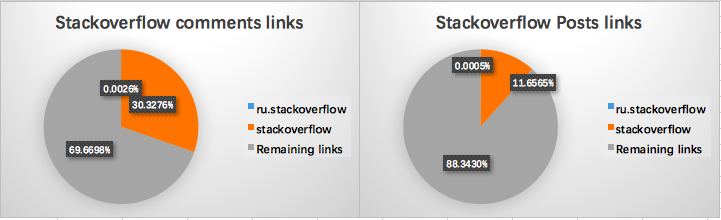
\includegraphics[width = 1.0\textwidth]{link3.png}
		\caption{Links in Stackoverflow}
  	\end{figure}
Similarly, for Russian Stackoverflow:
	\begin{figure}[H]
		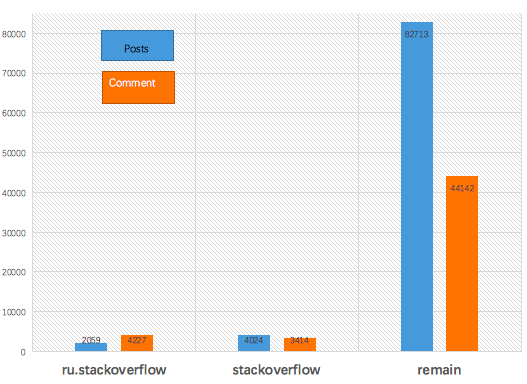
\includegraphics[width = 0.75\textwidth]{link1.png}
		\caption{Amount of links activily in Russian Stackoverflow}]
		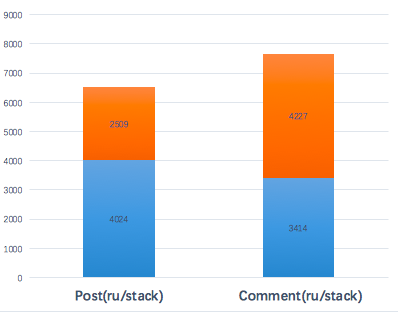
\includegraphics[width = 0.75\textwidth]{link2.png}
		\caption{Compare betweenthe amount of links to stackoverflow site and Russian subsite}
  	\end{figure}
Apparetly, in stackoverflow set, 12,220,205 posts used links in their body text. 11.66\% of them link to stackoverflow itself, while only 67 links are lead to Russian subsite. In Russian stackoverflow, 88,796 posts used links in theis body text. 4.53\% of them link to stackoverflow main site, while 2.32\% of them link to Russian subsite itself. The result of the link activities shows that Russian Stackoverlfow subsite is relatively independent community, which support itself by a lot of link activities instead of making the majority of their references to the main Stackoverflow site. However, in some ways the Russian Stackoverflow subsite has a non-negligible demand of knowledge refenrence to the main site according to the compare of destination between the amount of links.
		
	
\newpage
\section{Users}
It has been widely believed that users data is highly important for the community analysis. User activity can be revealed by data, which have already been structurized into different types. Hence, the analysis of user would be expanded with different aspects.
\\First of all, the intersection of these two sets is the foundation of this part of research, which is the users that owns th main site account and Russian subsite account at the same time. A point worth mentioning is that not only people from Russia use Russian for introduction and answers, but also some other countries like Ukraine and Belarus. That is the user base called "Russian Speakers".
\\Stackoverflow main site has 6,833,276 users, while Ru.stackoverflow has 65,623 users art the same time. Each stackexchange user account has a unique accountId, which is always the same if the user sign up for a subsite account like Russian or Spanish Stackoverflow. Using this information, the number of the intersection can be found as 35,751, which is nearly 54.48\% of the total number of users in Russian Stackoverflow. 
\subsection{CreationDate}
Focusing on this intersection user base, the user movement is calculated by their account creation date of each site. As the result shows in figure 4, 11,253 people have their Russian Stackoverflow account first and then sign up for a Stackoverflow account. While the other 24,498 users are the opposite of them. Here is the statistics for the users sign up Russian Stackoverflow in figure 5. Apparantly, the conclusion of this section is that user base is segregated by the new subsite and the number of users leaving the main site to their native language subsite is growing with the time goes by.
	\begin{figure}[H]
		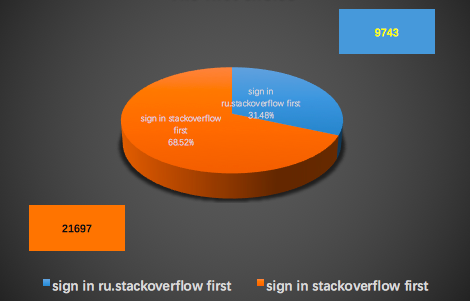
\includegraphics[width = 0.75\textwidth]{user2.png}
		\caption{Creation date compare}
		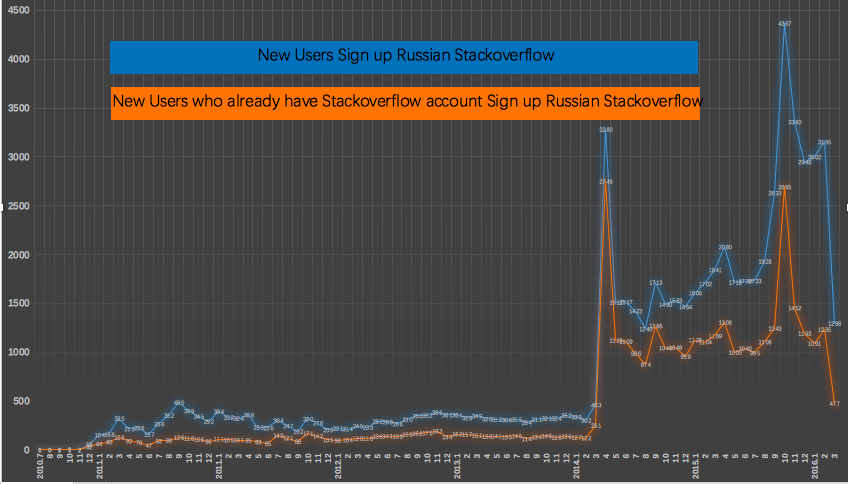
\includegraphics[width = 1.0\textwidth]{user1.png}
		\caption{User movement for signing up Russian Stackoverflow in each month}
  	\end{figure}

\subsection{Location and AboutMe}
Basically, all the users who can speak Russian can be found in a simple way. The Russian Alphabet can filter all the people using Russian in the main Stackoverflow site, and a list of location can be created at the same time, which can also be used to filter people who come from Russian-speaking areas. There must be an assumption that the user who come from a Russian-speaking location can speak Russian. In this way, 43,827 users can be seen as a set. Surprisingly, only 9,678 users of them have a Russian stackoverflow account, which means 77.92\% of these Russian speakers choose to use Stackoverflow site only.

\subsection{Reputation}
Reputation is a very valuable information that can be used to reveal the active level of users. The assumption is the user whose reputation is under 20 will be seen as an inactive user. As the result shows in figure 6, a huge number of inactive users, which includes a number of barely used accounts whose reputation is 1. And the remaining data shows there are more users’stackoverflow account owns a higher reputation than their Russian ones.
	\begin{figure}[H]
		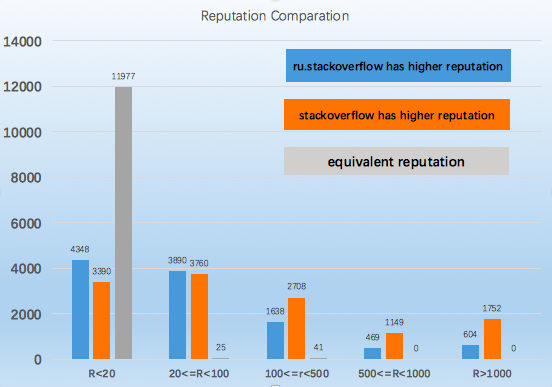
\includegraphics[width = 1.0\textwidth]{user3.png}
		\caption{Reputation compare}
  	\end{figure}
  	
\subsection{Post statistics}
In Stackoverflow main site, 12,472,796 out of 34,857,917 posts have been answered, which is 38.65\%. And in Russian Stackoverflow, 135,841 out of 310,539 posts have been answered, which is 43.74\%. Russian Stackoveflow clearly has a higher answer rate than Stackoverflow. For the intersection users base, the statistics of their posts are in figure 7.
	\begin{figure}[H]
		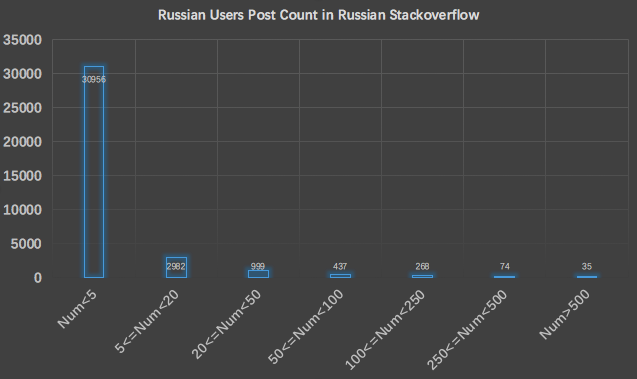
\includegraphics[width = 1.0\textwidth]{user4.png}
		\caption{The number of posts for users having both Russian stackoverflow account and Stackoverflow account}
  	\end{figure}


\end{document}
